% Attention Mechanism Template
% Self-attention or cross-attention diagram

\documentclass[tikz,border=8pt]{standalone}
\usepackage{tikz}
\usetikzlibrary{calc,positioning,fit,backgrounds}
\usepackage{amsmath}

\begin{document}
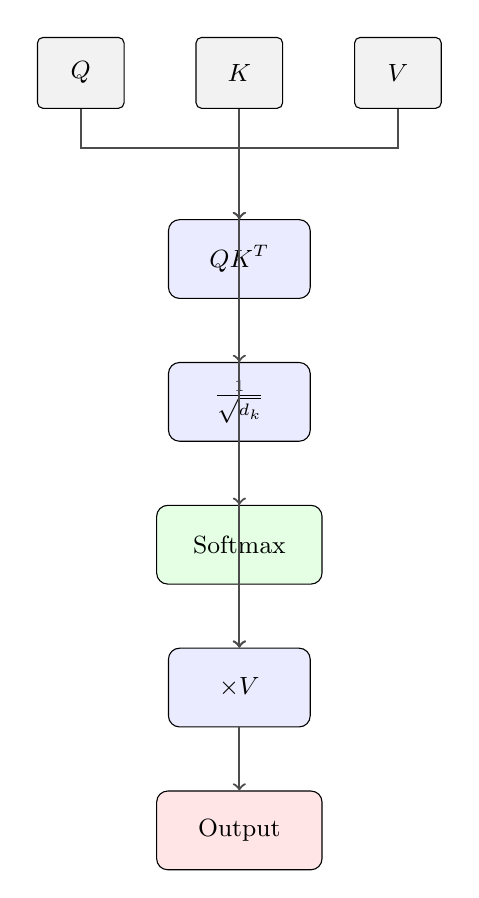
\begin{tikzpicture}[
    node distance=1.4cm,
    font=\small,
    % Node styles
    input/.style={draw, rounded corners=2pt, minimum width=1.1cm, minimum height=0.9cm, fill=gray!10},
    op/.style={draw, rounded corners=4pt, minimum width=1.8cm, minimum height=1cm, fill=blue!8},
    softmax/.style={draw, rounded corners=4pt, minimum width=2.1cm, minimum height=1cm, fill=green!10},
    output/.style={draw, rounded corners=4pt, minimum width=2.1cm, minimum height=1cm, fill=red!10},
    arrow/.style={->, thick, draw=black!70},
]

    % Q, K, V inputs
    \matrix[column sep=0.9cm] (inputs) {
        \node[input] (Q) {$Q$}; &
        \node[input] (K) {$K$}; &
        \node[input] (V) {$V$};   \\
    };
    
    % Attention computation
    \node[op, below=1.4cm of K] (scores) {$QK^T$};
    \node[op, below=0.8cm of scores] (scale) {$\frac{1}{\sqrt{d_k}}$};
    \node[softmax, below=0.8cm of scale] (softmax) {Softmax};
    \node[op, below=0.8cm of softmax] (weight) {$\times V$};
    \node[output, below=0.8cm of weight] (out) {Output};
    
    % Connections
    \draw[arrow] (Q.south) -- ++(0,-0.5) -| (scores);
    \draw[arrow] (K) -- (scores);
    \draw[arrow] (scores) -- (scale);
    \draw[arrow] (scale) -- (softmax);
    \draw[arrow] (softmax) -- (weight);
    \draw[arrow] (V.south) -- ++(0,-0.5) -| (weight);
    \draw[arrow] (weight) -- (out);

\end{tikzpicture}
\end{document}
